\documentclass{article}
\usepackage{tikz}
\usepackage{graphicx} % Required for inserting images
\usepackage{hyperref} % Required for inserting images
\usepackage{natbib}
\usepackage{amsmath,amsfonts,amsthm}
\usepackage{fullpage}
\usepackage{algpseudocode}
\usepackage{algorithm}
\usepackage{booktabs}
\usepackage{caption}
\usepackage{float}
\title{Isotonic Regression for Label Position Optimization}
\author{Toby Hocking}
\date{Nov 2026}

\DeclareMathOperator*{\argmin}{arg\, min} 
\DeclareMathOperator*{\argmax}{arg\, max} 
\begin{document}

\maketitle

\begin{abstract}
In a statistical graphic with several curves drawn in different colors, it is desirable to draw text labels at the end of the curves.
To ensure that the labels are readable, they should not overlap each other, and they should remain in the plotting region.
A previous solution to this label position optimization problem involves quadratic programming, which is cubic time and quadratic space in the number of labels.
We propose a new solution method, which involves a change of variables, reframing the problem as an isotonic regression, for which numerous efficient solvers exist.
We provide detailed comparisons of these previous solvers, in term of theoretical and empirical time and space complexity.
Our new algorithm has improved time and space complexity,  asymptotically linear, $O(n)$ for $n$ labels.
\end{abstract} 


\section{Introduction}
\begin{figure}
    \centering
    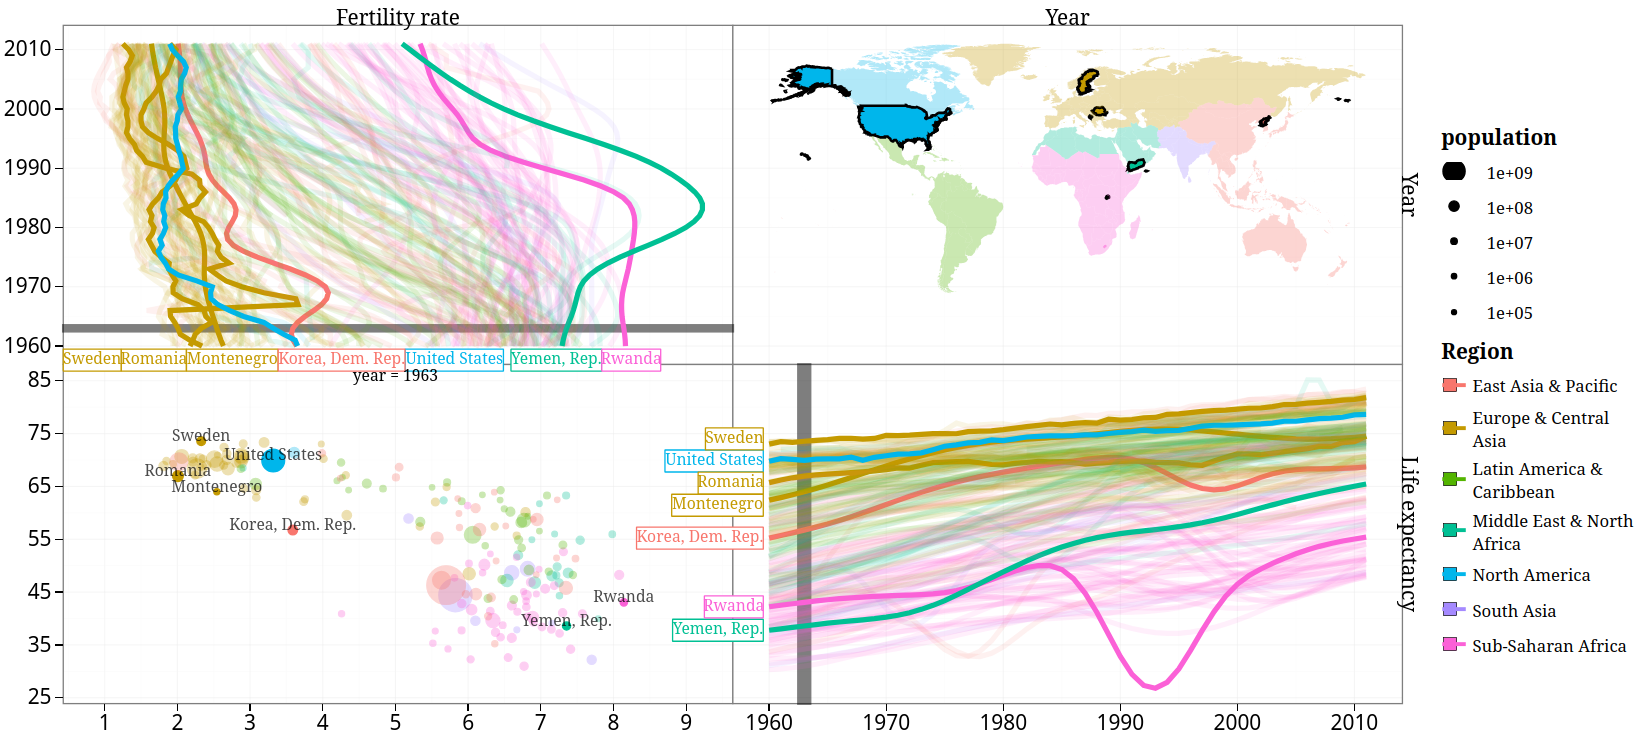
\includegraphics[width=\linewidth]{worldbank-labels.png}
    \caption{Caption}
    \label{fig:worldbank-labels}
\end{figure}

In a statistical graphic, different curves can be drawn to represent data from different sources.
For example, Figure~\ref{fig:worldbank-labels} shows 1960--2010 time series of data from the World Bank (life expectancy and fertility rate), with one curve per country.
The figure was created with R package animint2 \citep{Sievert2019jcgs, animint2}.
R packages like animint2 and directlabels \citep{directlabels} implement aligned text label drawing in a way that uses optimization to ensure readability.
In particular, the label is drawn as close as possible to the end of the corresponding curve, subject to two kinds of constraints.
First, none of the labels may be drawn outside of the plotting area.
For example, in the upper left panel of Figure~\ref{fig:worldbank-labels}, we see that the left border of the text label for Sweden is drawn at the far left of the plotting area.
Second, none on the labels may overlap each other.
For example, in Figure~\ref{fig:worldbank-labels}, we see that this constraint is obeyed for all of the labels drawn in the upper left and bottom right panels.

The subject of this paper is a new algorithm for efficiently computing such label positions.
This paper begins by describing the previous algorithm based on quadratic programming, which is relatively inefficient.
For $n$ labels, the previous algorithm is quadratic space, $O(n^2)$, and cubic time, $O(n^3)$.
This paper proposes a new algorithm that is asymptotically faster: linear time and space, $O(n)$.

\section{Related work}
R is a state-of-the-art free software system for statistical computing and graphics \citep{R}.
The quadprog R package \citep{quadprog} implements a dual algorithm for solving quadratic programming problems \citep{goldfarb1983numerically}.
Previously, \citet{de2009isotone} reviewed free software implementations of PAVA, but without comparison of computational complexity.
\citet{busing2022monotone} proposed a new linear time PAVA algorithm, including detailed comparisons with previous algorithms, in terms of thoretical and empirical time and space complexity.
Since August 2026, R package directlabels provides a dynamic programming algorithm for isotonic regression \citep{directlabels}.

\section{Problem}

\subsection{Data}

We assume there are $n$ labels.
Each label $i\in\{1,\dots,n\}$ has two associated data: a target position $t_i\in\mathbb R$, and a half-size $h_i\in\mathbb R_+$.
We assume the labels are already sorted by target value, $t_1\leq\cdots\leq t_n$.

Let $x_1,\dots,x_n$ be the label centers (optimization variables).
For each label $i$, the lower limit of its text is $x_i-h_i$, and the upper limit is $x_i+h_i$.
We assume the user inputs a global lower bound $\underline B\in\mathbb R$ and upper bound $\overline B\in\mathbb R$ in which text can be drawn.

\subsection{Optimization}

The label positions are determined as the solution of the optimization problem:
\begin{equation}
    \label{eq:label-pos}
\begin{aligned}
  \min_{x\in\mathbb R^n} & ||x-t||^2 \\
  \text{subject to }& x_1 - \underline B\geq h_1 ,\\
                    & \forall i\in\{2, \dots, n\},\, x_i-x_{i-1} \geq h_i + h_{i-1},\\
   & \overline B-x_n\geq h_n .
\end{aligned}
\end{equation}
\section{Solutions}

\subsection{Previous solution using quadratic programming}
TODO.
copy math and figure from

\url{https://tdhock.github.io/directlabels/HOCKING-useR-2011-directlabels-poster.pdf}


\subsection{Proposed solution using PAVA}

The proposed solution involves using a change of variables and PAVA.
First, let the lower limit vector be
\begin{equation}
  \label{eq:L}
  L = \texttt{cumsum}(\underline B+h_1, h_1+h_2, \dots, h_{n-1}+h_n).
\end{equation}
Each element of the $L$ vector represents the lower feasible limit of the corresponding element of $x$, given the constraints.
In other words, $L\in\mathbb R^n$ is a vector, with elements defined as
\begin{equation}
  \label{eq:L_i}
  L_i =
  \begin{cases}
    \underline B+h_1 & \text{ for } i=1\\
    L_{i-1}+h_{i-1}+h_i & \text{ for }i\in\{2,\dots, n\}.
  \end{cases}
\end{equation}
The change of variables is targets $d=t-L$, and solution $v=x-L$.
In this new space, the feasible set is $v_i\in [0, U]$ for all $i$, where the upper limit is $U=\overline B-h_n-L_n$.

The corresponding optimization problem is isotonic regression with bounds,
\begin{equation}
    \label{eq:pava-problem}
\begin{aligned}
  \min_{v\in\mathbb R^n} & ||v-d||^2 \\
  \text{subject to }& v_1 \geq 0 ,\\
                    & \forall i\in\{2, \dots, n\},\, v_{i-1} \leq v_{i},\\
   & v_n\leq U.
\end{aligned}
\end{equation}
By using the definitions of $d,v,L,U$, it can be shown that~(\ref{eq:pava-problem}) is equivalent to~(\ref{eq:label-pos}).

A simpler version of isotonic regression without bounds is
\begin{equation}
    \label{eq:no-bounds}
\begin{aligned}
 \min_{w\in\mathbb R^n} & ||w-d||^2 \\
  \text{subject to }& \forall i\in\{2, \dots, n\},\, w_{i-1} \leq w_{i}.\\
\end{aligned}
\end{equation}
Given a vector of data $d$, PAVA($d$) is an algorithm that computes $w$, the solution to~(\ref{eq:no-bounds}).
Because the isotonic regression objective is the squared difference between optimization variables and targets, the projection onto the feasible set $[0,U]$ can be computed by thresholding.
Therefore, after computing $w$, we compute $v = [ v_1, \dots, v_n ]$ with
\begin{equation}
    v_i = \begin{cases}
        0 & \text{ if } w_i < 0 \\
        U & \text{ if } w_i > U \\
        w_i & \text{ otherwise.}
    \end{cases}
\end{equation}

After computing the bounded isotonic regression solution $v$, the solution to~(\ref{eq:label-pos}) is computed via $x=v+L$.
Algorithm~\ref{alg:pava-pos} summarizes the solution method.

\begin{algorithm}
\begin{algorithmic}
  \Require half sizes $h_1,\dots,h_n\in\mathbb R$, target positions $t_1\leq\cdots\leq t_n\in\mathbb R$, bounds $\underline B<\overline B\in \mathbb R$.
  \State $L \gets \texttt{cumsum}(\underline B+h_1, h_1+h_2, \dots, h_{n-1}+h_n)$
  \State $U \gets \overline B-h_n-L_n$
  \State $v \gets \texttt{BoundedPAVA}(t-L, 0, U)$
  \State \Return $v+L$
\end{algorithmic}
  \caption{\label{alg:pava-pos}PAVA for label position optimization}
\end{algorithm}

\section{Justin}

\subsection{Algorithms covered}

The following table presents all the functions covered, as well as if they were mentioned in either \citet{de2009isotone} or in \citet{busing2022monotone}. For both columns, blank means they were not mentioned in the paper, and for the \citet{busing2022monotone} column, it is filled out with the $O$ time complexity that \cite{busing2022monotone} mentions in his paper for that function.

Functions that have \texttt{monotone::legacy(k)} in parentheses have an implementation both in the function we mention and in the \texttt{monotone} package. Functions that mention \texttt{monotone::legacy} first, they have no main implementation available in another package or GitHub repository.

\begin{table}[H]
    \centering
    \begin{tabular}{@{}lcc@{}}
        \toprule
        Function & \citet{de2009isotone} & \citet{busing2022monotone} \\
        \midrule
        \texttt{cir::oldPAVA()} & yes & \\
        \texttt{clue:::pava()} & yes & \\
        \texttt{density\_friendly\_pava()} (\texttt{monotone::legacy(12)}) & & $N$ \\
        \texttt{directlabels::isoreg\_dp()} & & \\
        \texttt{fdrtool::monoreg()} (\texttt{monotone::legacy(8)}) & yes & $N$ \\
        \texttt{Iso::pava()} (\texttt{monotone::legacy(6)}) & yes & $N^2$ \\
        \texttt{intcox:::intcox.pavaC()} & yes & \\
        \texttt{isotone::gpava()} & & \\
        \texttt{jbkpava()} (\texttt{monotone::legacy(14)}) & & $N$ \\
        \texttt{logcondens::isoMean()} & yes & \\
        \texttt{monotone::legacy(3)} (\texttt{amalgm()}) & & $N^2$ \\
        \texttt{monotone::legacy(1)} (\texttt{fitm()}) & & $N$ \\
        \texttt{monotone::legacy(11)} (\texttt{inplace\_pava()}) & & $N$ \\
        \texttt{monotone::legacy(10)} (\texttt{linear\_pava()}) & & $N^2$ \\
        \texttt{monotone::legacy(4)} (\texttt{pav()}) & & $N^2$ \\
        \texttt{monotone::legacy(9)} (\texttt{pooled\_pava()}) & & $N$ \\
        \texttt{monotone::monotone()} & & $N$ \\
        \texttt{orthoMTL::nnmaxheap\_C()} & & \\
        \texttt{SAGx::pava()} & yes & \\
        \texttt{quadprog::solve.QP()} & & \\
        \texttt{sandwich::pava.blocks()} & yes & \\
        \texttt{sffdr::monoSmooth\_pava()} & & \\
        \texttt{smacof:::pavasmacof()} (\texttt{monotone::legacy(2)}) & yes & \\
        \texttt{smacof:::wmonreg()} & & $N^2$ \\
        \texttt{stats::isoreg()} (\texttt{monotone::legacy(5)}) & yes & $N^2$ \\
        \texttt{spsurvey::isotonic()} (\texttt{monotone::legacy(7)}) & & $N^2$ \\
        \texttt{TabICL2:::.pava\_single()} & & \\
        \texttt{toxstats:::pava()} & & \\
        \texttt{UniIsoRegression::reg\_1d()} (\texttt{monotone::legacy(13)}) & & $N$ \\
        \bottomrule
    \end{tabular}
    \caption{Functions benchmarked and whether they appear in \citet{de2009isotone} and \citet{busing2022monotone}.}
    \captionsetup{font=footnotesize}
    \caption*{\centering \texttt{monotone::legacy(k)} stands for \texttt{monotone::legacy(number = k)}.}
    \label{tab:paper-comparison}
\end{table}

\subsection{Analysis}

\subsubsection{Data used}
The algorithm comparisons that are shown in the next few graphs use data that are generated using 6 different methods. They are as follows:

\begin{table}[H]
    \centering
    \begin{tabular}{lll}
        \toprule
        Description & Equation & \textsf{R} code \\
        \midrule
        Up-down & $x_i = \min(i,\, n - i + 1)$                 & \verb|x <- c(1:(n / 2), (n / 2):1)| \\
        Up      & $x_i = i$                                    & \verb|x <- 1:n| \\
        Down    & $x_i = n - i + 1$                            & \verb|x <- n:1| \\
        Cliff   & $x_i = i$ for $i < n$, \; $x_n = -n^2$       & \verb|x <- c(seq_len(n - 1), -n^2)| \\
        Zigzag  & $x_i = i \bmod 2$                            & \verb|x <- rep_len(c(1, 0), n)| \\
        Normal  & $x_i \sim \mathcal{N}(0, 1)$                 & \verb|x <- rnorm(n)| \\
        \bottomrule
    \end{tabular}
    \caption{Data-generating functions}
    \label{tab:generators}
\end{table}

We used these data-generating functions for the following reasons: 
\begin{itemize}
    \item Up-down: a first half without violations followed by a decreasing second half, to catch algorithms that are slow at reaching back into blocks they had already accepted
    \item Up: usually the best case, as the data is already in order and there are no merges to do
    \item Down: usually the worst case, as everything is a violation (when you walk forward) and you end up with a single block. For some functions, such as \texttt{stats::isoreg()}, it is instead the best case scenario (as they walk backward)
    \item Cliff: increasing data with a single very low final value, which forces all existing blocks to merge at once. It was originally meant to catch algorithms that could be programmed in an unsafe way, such as \texttt{sandwich::pava.blocks()}, which produces a stack overflow with it starting around N = 2500
    \item Zigzag: a violation at every second value, each resolved locally, which produces many small blocks with tied means
    \item Normal: random, unstructured data, as a stand-in for the average case.
\end{itemize}

\subsubsection{Errors seen while testing}

\begin{itemize}
    \item The \texttt{sandwich::pava.blocks()} function, with the cliff dataset, as described earlier, produces a stack overflow (\texttt{Error: node stack overflow}) from around $N=2500$.
    \item Both the \texttt{UniIsoRegression::reg\_1d} and \texttt{monotone::legacy(13)} (the latter being an implementation of the earlier in the \texttt{monotone} package) have errors:
    \begin{itemize}
        \item The original version seems to count the first element twice whenever a pooled block reaches the start of the vector. This seems to be corrected in the \texttt{monotone::legacy} function, but makes the original wrong whenever a pooled block reaches the first element.
        \item The legacy version initializes a vector with all zeros, (\texttt{mean\_vec}) and never sets it out to what it is supposed to be originally (\texttt{x}). This causes values that are already in order, in some cases, to be pooled together, becoming wrong whenever the data has values that should not be pooled.
    \end{itemize}
    \item \texttt{orthoMTL::nmaxheap\_C()} on version 0.1.0 gives wrong results whenever a pooled block has a single element, even on data that is already in order. This is fixed in version 0.1.1, after a comment was left in their repository.
\end{itemize}

\subsubsection{Results summary}

Validation here was done against \texttt{quadprog::solve.QP()}. We assume it to be the source of truth, and most results (all except the errors noted in the previous section) match this function's results. As \texttt{quadrpog::solve.QP()} is quite slow, it does not test all the values of the functions, but we assume if the first few thousand results are equal, the next ones will be as well. These results are equal up to a tolerance of approximately $1.5\times10^{-8}$ (as we use \href{https://www.rdocumentation.org/packages/base/versions/3.6.2/topics/all.equal}{all.equal} to compare).
% TOOD JUSTIN: Mention that scipy and scikit learn use the same C code (see if corresponds to R)
% TODO JUSITN: add table 2 busing with only our O(N) functions, adding everything that was not previously there
% TODO JUSTIN: remove orthomtl 0.1.0, rerun everything with version 0.1.1
% TODO JUSTIN: donner quelques exemples, dire tel algo est meilleur et pire sur up et down, et l'autre est meilleur et pire sur down et up. Donner exemple lineaire les deux cas. dire qu'on va particulierement s'interesser a ceux qui marchent particulierement dans tous les cas
% TODO JUSTIN: add graphique with one line linear, one line quadratic, one line cubic, with like quadprog, stats, monotone::monotone
% TODO JUSTIN: add graphique with like 5 best, after doing table 2 busing, choose the 5 best, plot them, compare them (figure pred)

% TODO JUSTIN: remove best space, best time, say that they were all O(N), and combine table 1 and table 3 (functions.md and paper comparison)
% TODO JUSTIN: put alternating colors lines
% TODO JUSTIN: 4 categories: n2 time & space, n2 time n space, quadprog, n time n space, separated by lines. mention that it is consistent with Busing
% TODO JUSTIN: add quadprog to results table
% TODO JUSTIN: remarquer dynamic programming pour quadprog and directlabels
% TODO JUSTIN: for UniIsoRegression, add star saying it errors, give two examples about the errors
% TODO JUSTIN: remove everything from the paper that was not in CRAN


\begin{table}[H]
    \centering
    \begin{tabular}{@{}lccccc@{}}
        \toprule
        Function & Best space & Worst space & Best time & Worst time & \citet{busing2022monotone} \\
        \midrule
        \texttt{cir::oldPAVA()} & $N$ & $N^2$ & $N\log N$ & $N^2$ & \\
        \texttt{clue:::pava()} & $N\log N$ & $N^2$ & $N$ & $N^2$ & \\
        \texttt{density\_friendly\_pava()} & $N$ & $N\log N$ & $N$ & $N\log N$ & $N$ \\
        \texttt{directlabels::isoreg\_dp()} & $N$ & $N\log N$ & $N$ & $N\log N$ & \\
        \texttt{fdrtool::monoreg()} & $N$ & $N\log N$ & $N$ & $N\log N$ & $N$ \\
        \texttt{intcox:::intcox.pavaC()} & $N$ & $N\log N$ & $N$ & $N\log N$ & \\
        \texttt{Iso::pava()} & $N$ & $N$ & $N$ & $N^2$ & $N^2$ \\
        \texttt{isotone::gpava()} & $N\log N$ & $N^2$ & $N$ & $N^2$ & \\
        \texttt{jbkpava()} & $N$ & $N\log N$ & $N$ & $N\log N$ & $N$ \\
        \texttt{logcondens::isoMean()} & $N$ & $N$ & $N$ & $N$ & \\
        \texttt{monotone::monotone()} & $N$ & $N\log N$ & $N$ & $N\log N$ & $N$ \\
        \texttt{monotone::legacy(3)} (\texttt{amalgm()}) & $N$ & $N\log N$ & $N$ & $N^2$ & $N^2$ \\
        \texttt{monotone::legacy(1)} (\texttt{fitm()}) & $N$ & $N\log N$ & $N$ & $N\log N$ & $N$ \\
        \texttt{monotone::legacy(11)} (\texttt{inplace\_pava()}) & $N$ & $N\log N$ & $N$ & $N\log N$ & $N$ \\
        \texttt{monotone::legacy(10)} (\texttt{linear\_pava()}) & $N$ & $N\log N$ & $N$ & $N^2$ & $N^2$ \\
        \texttt{monotone::legacy(4)} (\texttt{pav()}) & $N$ & $N\log N$ & $N$ & $N^2$ & $N^2$ \\
        \texttt{monotone::legacy(9)} (\texttt{pooled\_pava()}) & $N$ & $N\log N$ & $N$ & $N\log N$ & $N$ \\
        \texttt{orthoMTL::nnmaxheap\_C()} & $N$ & $N$ & $N$ & $N$ & \\
        \texttt{SAGx::pava()} & $N$ & $N^2$ & $N$ & $N^2$ & \\
        \texttt{sandwich::pava.blocks()} & $N$ & $N^2$ & $N$ & $N^2$ & \\
        \texttt{sffdr::monoSmooth\_pava()} & $N$ & $N\log N$ & $N$ & $N\log N$ & \\
        \texttt{smacof:::pavasmacof()} & $N$ & $N^2$ & $N$ & $N^2$ & \\
        \texttt{smacof:::wmonreg()} & $N$ & $N$ & $N$ & $N^2$ & $N^2$ \\
        \texttt{spsurvey::isotonic()} & $N$ & $N^2$ & $N$ & $N^2$ & $N^2$ \\
        \texttt{stats::isoreg()} & $N$ & $N\log N$ & $N$ & $N^2$ & $N^2$ \\
        \texttt{TabICL2:::.pava\_single()} & $N$ & $N$ & $N$ & $N$ & \\
        \texttt{toxstats:::pava()} & $N$ & $N$ & $N$ & $N\log N$ & \\
        \texttt{UniIsoRegression::reg\_1d()} & $N$ & $N\log N$ & $N$ & $N\log N$ & $N$ \\
        \bottomrule
    \end{tabular}
    \caption{\centering Empirical best- and worst-case space and time complexity of the functions benchmarked, alongside the time complexity reported by \citet{busing2022monotone}, in $O$ notation.}
    \captionsetup{font=footnotesize}
    \caption*{\centering \texttt{monotone::legacy(k)} stands for \texttt{monotone::legacy(number = k)}.}
    \label{tab:complexity}
\end{table}




\appendix
\subsection{Appendix}

\subsubsection{Function versions}

These are the versions of the functions we have used, as so to easily reproduce the results we have presented here.

\begin{table}[H]
    \centering
    \begin{tabular}{@{}lll@{}}
        \toprule
        Function & Version & Date \\
        \midrule
        \texttt{cir::oldPAVA()} & 2.5.1 & 2025-02-01 \\
        \texttt{clue:::pava()} & 0.3-68 & 2026-03-26 \\
        \texttt{density\_friendly\_pava()}$^{**}$ & -- & 2016-05 \\
        \texttt{directlabels::isoreg\_dp()} & 2026.8.27 & 2026-08-28 \\
        \texttt{fdrtool::monoreg()} & 1.2.18 & 2024-08-20 \\
        \texttt{intcox::intcox.pavaC()} & 0.9.3 & 2013-02-25 \\
        \texttt{Iso::pava()} & 0.0-21 & 2023-10-02 \\
        \texttt{isotone::gpava()} & 1.1-2 & 2025-05-22 \\
        \texttt{jbkpava()}$^{**}$ & -- & -- \\
        \texttt{logcondens::isoMean()} & 2.1.9 & 2026-04-26 \\
        \texttt{monotone::legacy()} & 0.1.2 & 2022-05-25 \\
        \texttt{monotone::monotone()} & 0.1.2 & 2022-05-25 \\
        \texttt{orthoMTL::nnmaxheap\_C()}$^{***}$ & 0.1.0 & 2026-08-07 \\
        \texttt{quadprog::solve.QP()} & 1.5-8 & 2019-11-20 \\
        \texttt{SAGx::pava()} & 1.64.0 & 2020-10-27 \\
        \texttt{sandwich::pava.blocks()} & 3.1-3 & 2026-08-03 \\
        \texttt{sffdr::monoSmooth\_pava()} & 1.1.2 & 2026-03-31 \\
        \texttt{smacof:::pavasmacof()} & 2.1-7 & 2024-10-10 \\
        \texttt{smacof:::wmonreg()} & 2.1-7 & 2024-10-10 \\
        \texttt{spsurvey::isotonic()} & 4.1.4 & 2020-09-18 \\
        \texttt{stats::isoreg()}$^{*}$ & 4.6.1 & 2026-06-24 \\
        \texttt{TabICL2:::.pava\_single()}$^{***}$ & -- & 2026-08-18 \\
        \texttt{toxstats:::pava()}$^{***}$ & -- & 2026-09-01 \\
        \texttt{UniIsoRegression::reg\_1d()} & 0.0-0 & 2017-11-07 \\
        \bottomrule
    \end{tabular}
    \caption{Versions of the functions benchmarked}
    \label{tab:versions}
    \captionsetup{font=footnotesize}
    \caption*{
        $^{*}$ Part of base R: the version and date are those of R itself.
        
        $^{**}$ Not a package: a source file copied into our repository on 2026-10-09, so it has no version. From \href{https://github.com/maxdan94/Density-Friendly/blob/master/exactDF.cpp}{\texttt{density\_friendly\_pava()}'s GitHub} and from \href{https://rpubs.com/deleeuw/262795}{\texttt{jbkpava()}'s RPubs page}.

        $^{***}$ A package, but only available on GitHub and not on CRAN: the date is that of the installed commit (\href{https://github.com/Novartis/orthoMTL/commit/dc91503391c820bb4589fe13afa7e517e8beb542}{orthoMTL \texttt{dc91503}}, \href{https://github.com/cregouby/TabICL2/commit/c1fee55af5362914f89e3b1b020e1f68dea9e90e}{TabICL2 \texttt{c1fee55}}, \href{https://github.com/open-AIMS/toxstats/commit/4bc579a139c9de0a6c523907bb9604e6f4a0dd11}{toxstats \texttt{4bc579a}}).
    }
\end{table}



\bibliographystyle{abbrvnat}
\bibliography{refs}

\end{document}
